% SPI API


% Indledning 

SPI kommunikationen har en API klasse på Master skrevet i \verb+C+++ og en handler på Enhed skrevet i \verb+C+.

For at add-on printet på Devkit8000 kan bruge GPIO benene til SPI kommunikationen er det nødvendigt at rute dem korrekt, dette gøre ved at bruge følgende 2 kommandoer.

\begin{itemize}
\item \verb+echo 0x3 > /sys/class/cplddrv/cpld/spi_route_reg+
\item \verb+echo 0x1 > /sys/class/cplddrv/cpld/ext_serial_if_route_reg+
\end{itemize}

Kernemodulet skal også indsættes og oprette en system node, i APIen bruges \verb+/dev/spi_dev+ så denne er fast.
Alt dette er skrevet i et shell script der håndtere alt indsætning og oprettelse af kernefilen, se bilag \verb+insert_SPI_dev.sh+

% SPI API

\subsection{SPI API}
% SPI API

SPI\_api er en klasse til at styre SPI kommunikationen. Den består af en række metoder beskrevet i afsnit \ref{fig:SPI API klassediagram}.

Alle metoderne er stort set opbygget ens.

\subsubsection*{Open}

De har alle en \verb+open()+ metode der sørger for at åbne system filen der enten skal skrives til eller læses fra. Hvis der sker en fejl i open, returnere den så en passende negativ fejl, i dette tilfælde fejlen LOG\_ERR.

\begin{lstlisting}[language=C]
/* Open file */
fp = open("/dev/spi_dev", O_RDWR);
if(fp < 0){
	printf("OPEN ERROR: %d\n", fp);
	close(fp);
	return -LOG_ERR;
}
\end{lstlisting}

\subsubsection*{Close}

Der er også altid en \verb+close()+ metode, der sørger for at lukke den åbnede fil ned igen. Denne metode er også lagt i alt fejlhåndtering, for at undgå systemfejl på Masteren, hvis der skulle ske fejl.



\begin{lstlisting}[language=C]
/* Close file */
close(fp);
\end{lstlisting}

\subsubsection*{Write \& Read}

Ind i mellem disse er så en \verb+write()+ eller/og en \verb+read()+ metode, der sørger for at der bliver læst fra eller skrevet til Enheden via SPI. Her er nogle eksempler på metoderne.

\verb+Write()+ metoden bruges i starten af alle metoder til at vælge hvad der skal ske på Enheden ved at skrive en char kommando til den. Den bruges også, som her, til at skrive parametrene temp og humi til Enheden. Her modtages parametrene som floats, konverteres til chars og skrives enkeltvis til Enheden med en for-løkke.

\begin{lstlisting}[language=C]
int SPI_api::config(int unit, float temp, float humi)
{
char tempArray[6];	// T T T . T \0
char humiArray[4];	// F F F \0

/* Parse floats to CharArrays */
snprintf(tempArray, sizeof(tempArray), "%05.1f", temp);
snprintf(humiArray, sizeof(humiArray), "%03.0f", humi);
..
..
..
/* Write temp to target without 0-termination */
for(int i = 0 ; i < 5 ; i++){
	err = write(fp, &tempArray[i], dataLen);
		if(err < 0){
		printf("WRITE ERROR: %d\n", err);
		close(fp);
		return -CONF_ERR;
	}
}

/* Write humidity to target without 0-termination */	
for(int i = 0 ; i < 3 ; i++){		
	err = write(fp, &humiArray[i], dataLen);
	if(err < 0){
		printf("WRITE ERROR: %d\n", err);
		close(fp);
		return -CONF_ERR;
	}
}
..
..
}
\end{lstlisting}

\verb+Read()+ metoden modtager chars fra Enheden og behandler dem. I koden nedenfor ses implementeringen for \verb+getLog()+ metoden som læser på en buffer på Enheden hvori der ligger Data og Fejl. Disse chars bliver så lagt i en vector<string> så programmet på Masteren har en nem måde at håndtere fejl og log-data på. Vector og alle string variablerne nulstilles med \verb+clear()+ for en god ordens skyld, da der nødigt skulle stå noget forkert i dem inden de pushes med ny data.

Den første \verb+read()+ metode man støder på, læser bufferlængden fra Enheden, som der sørger for der ikke læses på noget data der ikke er tilstede, senere i metoden.

Så er der en for-løkke der starter med at kigge på om der er et 'D' for data eller 'E' for fejl. Disse laver hhv. 10 og 3 læsninger, som der bygges en string af, der pushes til en vector. Hvis der kommer et 'D' ligges det på den første plads i en string sammen med de næste 10 læsninger. Dette er tilsvarende ved en fejl, dog kun med 3 læsninger efter det læste 'E'.

\begin{lstlisting}[language=C]
int SPI_api::getLog(vector<string> &data, int * units, int size)
{
..
..
..
char charArrayLen;		// Variable for charArray size from target
char charResult;		// Used for buffering read chars
string stringResult;
	stringResult.clear();
string stringDataResult;
	stringDataResult.clear();
string stringErrorResult;
	stringErrorResult.clear();
vector<string> vectorResult;
	vectorResult.clear();
..
..
..

/* Read charArray length from target */
err = read(fp, &charArrayLen, dataLen);
if(err < 0){
	printf("READ ERROR: %d\n", err);
	close(fp);
	return -LOG_ERR;
}
	
/* Vector Builder looking for D's or E's */
for(i = 1 ; i < charArrayLen ; i++){
	err = read(fp, &charResult, dataLen);
	if(err < 0){
		printf("READ ERROR: %d\n", err);
		close(fp);
		return -LOG_ERR;
	}

	if(charResult == 'D'){
		stringDataResult.push_back(charResult); // Push 'D' to stringDataResult
		
		// Build rest of stringDataResult
		for(int c = 0 ; c < dataStringLen ; c++){
			err = read(fp, &charResult, dataLen);
			if(err < 0){
				printf("READ ERROR: %d\n", err);
				close(fp);
				return -LOG_ERR;
			}			
			stringDataResult.push_back(charResult);
			
			// Error handling, prevent to read on non-existing data
			if(i >= (charArrayLen-1)){
				printf("Error in buffer from unit\n");
				return -LOG_ERR;
			}
			i++;	// Increment 1st for-loop counter
		}
		
		// Push string to vectorResult
		vectorResult.push_back(stringDataResult);
		stringDataResult.clear();
	}
	
	if(charResult == 'E'){
		stringErrorResult.push_back(charResult); // Push 'E' to stringErrorResult
		
		// Build rest of stringErrorResult
		for(int c = 0 ; c < errorStringLen ; c++){
			err = read(fp, &charResult, dataLen);
			if(err < 0){
				printf("READ ERROR: %d\n", err);
				close(fp);
				return -LOG_ERR;
			}
			stringErrorResult.push_back(charResult);

			// Error handling, prevent to read on non-existing data
			if(i >= (charArrayLen-1)){
				printf("Error in buffer from unit\n");
				return -LOG_ERR;
			}
				i++;	// Increment 1st for-loop counter
		}

		// Push string to vectorResult and clear string
		vectorResult.push_back(stringErrorResult);
		stringErrorResult.clear();
	}
}
\end{lstlisting}

\subsubsection*{Clear buffer}

Alle metoderne har også en Clear buffer funktion. Denne benytter \verb+write()+ metoden, til at skrive et 'C' til Enheden for at nulstille tx-bufferen. Den bruges også for at tilgå switchen for alle write-only metoderne.

\begin{lstlisting}[language=C]
/* Clear buffer */
err = write(fp, &CL_BUF, 1);
if(err < 0){
	printf("CLEAR ERROR: %d\n", err);
	close(fp);
	return -CONF_ERR;
}
\end{lstlisting}

Resten af implementeringen findes i bilag.


% SPI HANDLER

\subsection{SPI Handler}
% SPI Handler

\subsubsection*{Top-design - PSoC Creator 3.0}

Topdesignet (figur\ref{lab:topdesign_spi}( består af en SPI blok, samt 3 digitale output pins. Herunder beskrives hvordan elementerne i topdesignet skal indstilles.

\begin{figure}[H] \centering
{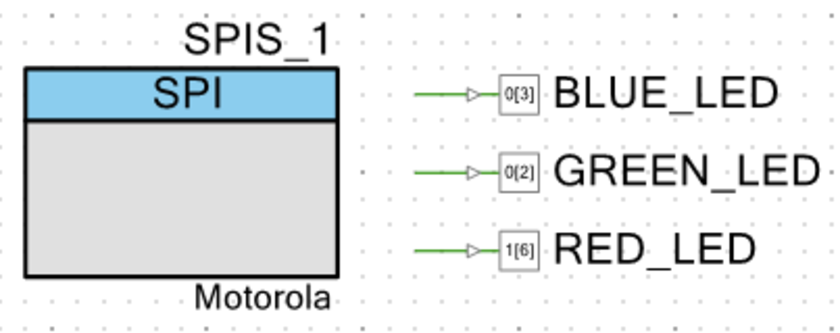
\includegraphics[width=0.4\textwidth]{filer/implementering/spi/spi_handler_topdesign}}
\caption{Topdesign for SPI og led}
\label{lab:topdesign_spi}
\raggedright
\end{figure}

Basis indstillingerne for SPI blokken ses i figur \ref{lab:spi_basic_config}. Mode sættes til slave, og SCLK mode sættes til CPOL=0, CPHA=0.

\begin{figure}[H] \centering
{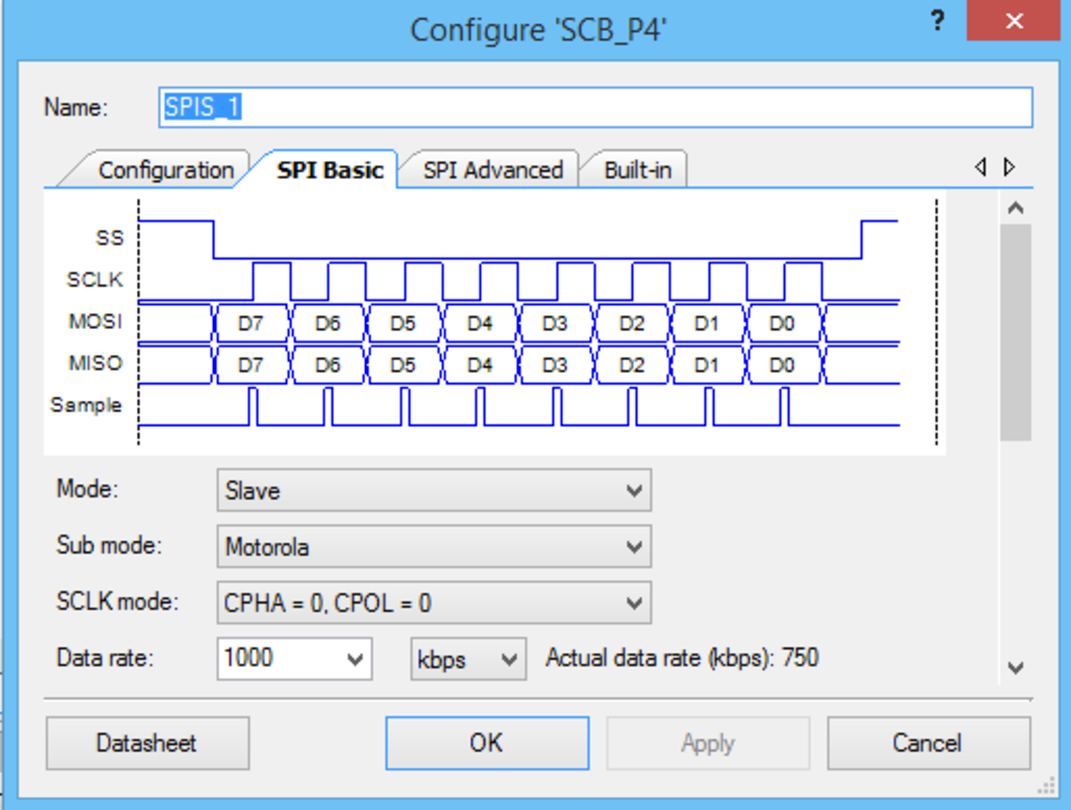
\includegraphics[width=0.8\textwidth]{filer/implementering/spi/spi_handler_topdesign_spi_basic}}
\caption{Konfigurering af SPI (SPI basic)}
\label{lab:spi_basic_config}
\raggedright
\end{figure}

De avancerede indstillinger for SPI blokken ses i figur \ref{lab:spi_advanced_config}. Buffer size sættes til 8 bit for både RX og TX. Interruptet sættes til internt og interrupt kilden er RX FIFO not empty og RX FIFO full.

\begin{figure}[H] \centering
{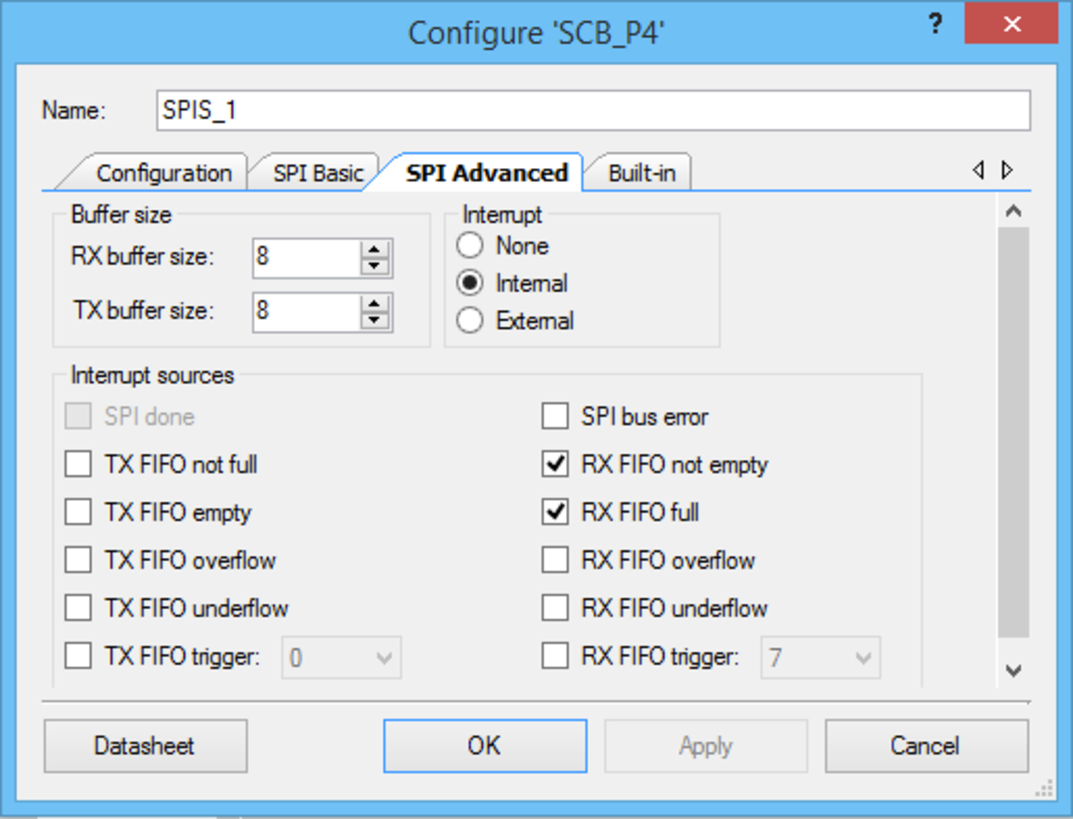
\includegraphics[width=0.8\textwidth]{filer/implementering/spi/spi_handler_topdesign_spi_advanced}}
\caption{Konfigurering af SPI (SPI advanced)}
\label{lab:spi_advanced_config}
\raggedright
\end{figure}

De 3 output pins (GREEN\_LED, BLUE\_LED, RED\_LED) skal sættes til digital output uden hardware connection.
Figur \ref{lab:led_pins_config} viser hvordan indstillingen skal være, dette er gældende for alle 3 pins. 

\begin{figure}[H] \centering
{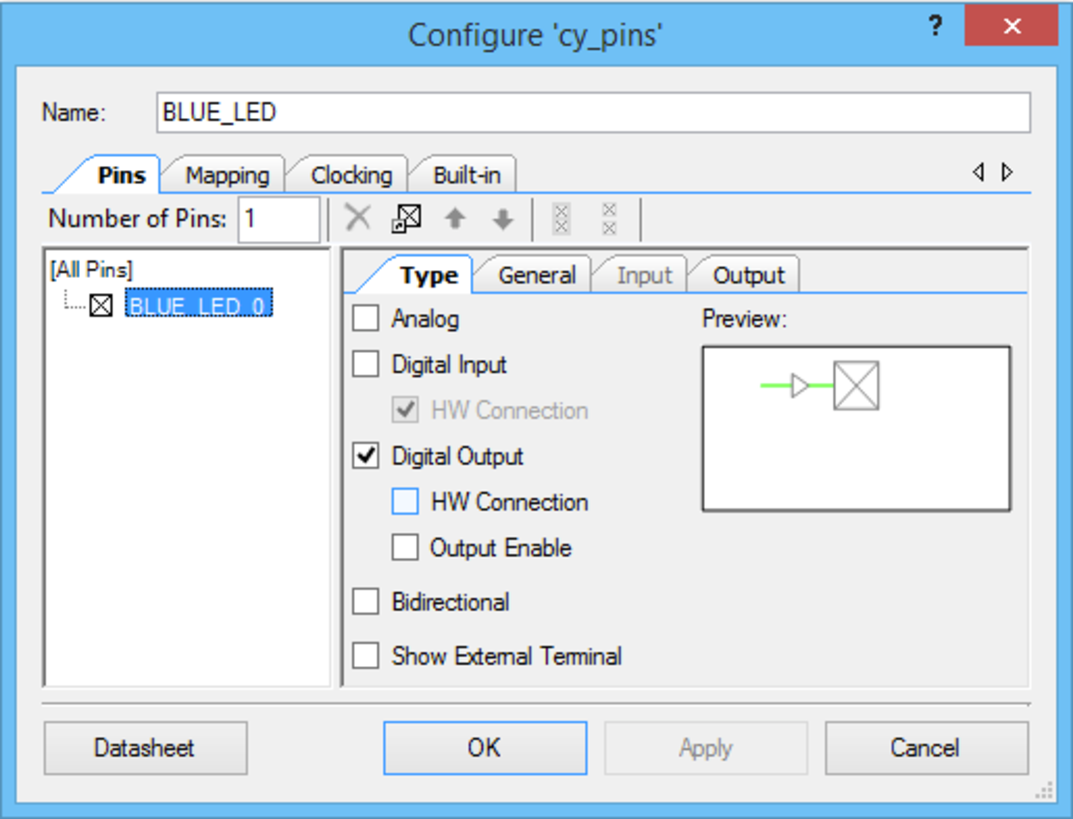
\includegraphics[width=0.8\textwidth]{filer/implementering/spi/spi_handler_topdesign_led}}
\caption{Konfigurering af pins}
\label{lab:led_pins_config}
\raggedright
\end{figure}


\subsubsection*{ISR}

SPI handleren består stort set kun af én interrupt rutine. Der tages udgangspunkt i de vigtige dele af rutinen. Og resten af koden kan ses i bilag.

Selve interrupt-rutinen er bygget op med en switch, der vælger en case alt efter input fra Masteren. Der tilgås kun switchen hvis der kommer en kommando der skal svare tilbage til Master (\verb+'R','L','V'+) eller en Clear buffer kommando \verb+'C'+, derefter kigges der på plads [0] i spiBuffer arrayet, og handles alt efter hvad der står der. Dvs. hvis Enheden skal aktiveres, sendes først et \verb+'A'+ fra Master som læses ind i spiBuffer[] arrayet efterfulgt af et \verb+'C'+ som tilgår switchen.
 
\begin{lstlisting}[language=C]
char spiBuffer[64];
..
..
..
CY_ISR(isr_spi_rx) {

	char cmd = '0';
	..
	.. 
	cmd = SPIS_1_SpiUartReadRxData(); 
    
    spiBuffer[spiCounter] = cmd;
    spiCounter++;
..
..
    if ((cmd == 'R') || (cmd == 'C') || (cmd == 'L') || (cmd == 'V')){
    	switch (spiBuffer[0]) {
\end{lstlisting}

Alle kommandoer der kræver et svar tilbage på SPI, bruger \verb+'R'+ casen, men eftersom PSoC4 kræver noget tid til at hente og skrive i tx-bufferen er koden lavet sådan at man er på forkant med en læsning. Dvs. når der laves en læsning \verb+'R'+ fra Masteren, er der allerede skrevet til tx-bufferen, så man reelt læser data ud med det samme. 

Det er derfor switchen tilgåes ved alle ''Read'' kommandoer, så hvor der f.eks. skal verificeres, laves der en læsning af Enhedens enhedsnummer. I eksemplet nedenfor er en global char brugt som enhedsnummer, denne læses ind i tx-bufferen når case \verb+'V'+ køres. Og når så case \verb+'R'+ køres, læses unitNo variablen først, hvorefter der skrives en ny værdi ind i tx-bufferen til næste \verb+'R'+ køres.

\begin{lstlisting}[language=C]
char unitNo = '1';
int spiCounter = 0;
int spiReadCounter = 0;
..
..
..
CY_ISR(isr_spi_rx) {
..
..
..
    		case 'V':
					..
					..
					..
                    SPIS_1_SpiUartClearTxBuffer();
                    SPIS_1_SpiUartWriteTxData(unitNo);
                    spiCounter = 0;
    			break;
..
..
..
            case 'R':
                    SPIS_1_SpiUartClearTxBuffer();
                    SPIS_1_SpiUartWriteTxData(spiTxBuffer[spiReadCounter]);
                    spiCounter = 0;
                    spiReadCounter++;
                break;
\end{lstlisting}


